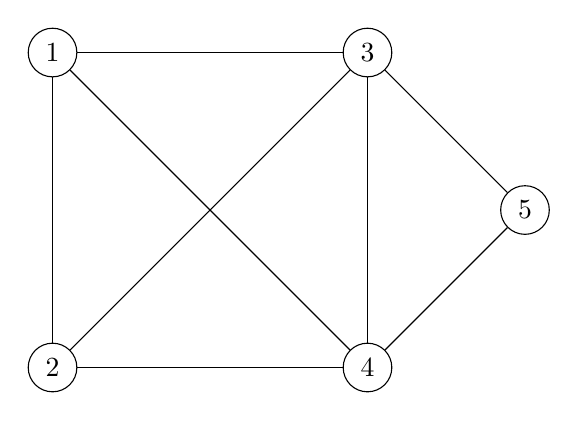
\begin{tikzpicture}[yscale=-1,scale=2]
\node[draw=black,circle] (N01) at (0,0) {1};
\node[draw=black,circle] (N02) at (0,2) {2};
\node[draw=black,circle] (N03) at (2,0) {3};
\node[draw=black,circle] (N04) at (2,2) {4};
\node[draw=black,circle] (N05) at (3,1) {5};
\draw (N01) -- (N02);
\draw (N01) -- (N03);
\draw (N01) -- (N04);
\draw (N02) -- (N03);
\draw (N02) -- (N04);
\draw (N03) -- (N04);
\draw (N03) -- (N05);
\draw (N04) -- (N05);
\end{tikzpicture}